\documentclass {article}

\usepackage{geometry}
\geometry {
 	a4paper,
 	total={210mm,297mm},
 	left=20mm,
 	right=20mm,
 	top=20mm,
 	bottom=20mm,
 }

\usepackage{fancyhdr}
\pagestyle{fancy}
\fancyhf{}
\rhead{}
\lhead{Beginner's Guide For Domjudge}
\rfoot{Page \thepage}

\usepackage {hyperref, amsmath, amsthm, amssymb, graphicx, tabularx}
\everymath {\displaystyle}

\newtheorem {theorem}{Theorem}
\newtheorem*{theorem*}{Theorem}

\newcommand{\define}{\newcommand}
\define{\set}[1]{\{{#1}\}}

\define{\img}[2]{{\begin{center}\includegraphics[scale={#1}]{{#2}}\end{center}}}


\begin {document}

\tableofcontents

\newpage
\section{DOMjudge}
\subsection{Overview}
DOMjudge is the online judge we use to host contests.

Go to \url{http://domjudge2.cs.illinois.edu/team/} and enter your assigned 
credentials to access the contest dashboard.

\begin{center}
    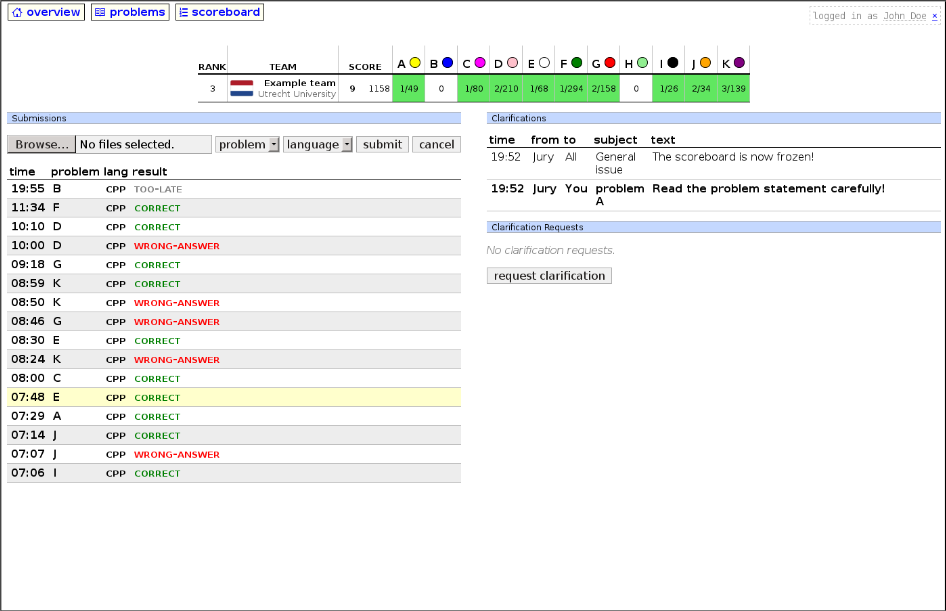
\includegraphics[scale=0.3]{dashboard.png}
\end{center}

On this page, you can
\begin{itemize}
\item view problem statements by clicking the problem names.
\item view the list of past submissions and verdicts (more about verdicts
      later).
\item upload your solution.
\item view and request clarification to problems.
\end{itemize}

\subsection{Scoreboard}
By clicking the \textbf{scoreboard} link on the top of the overview page, you
can access the scoreboard page. 

\begin{center}
    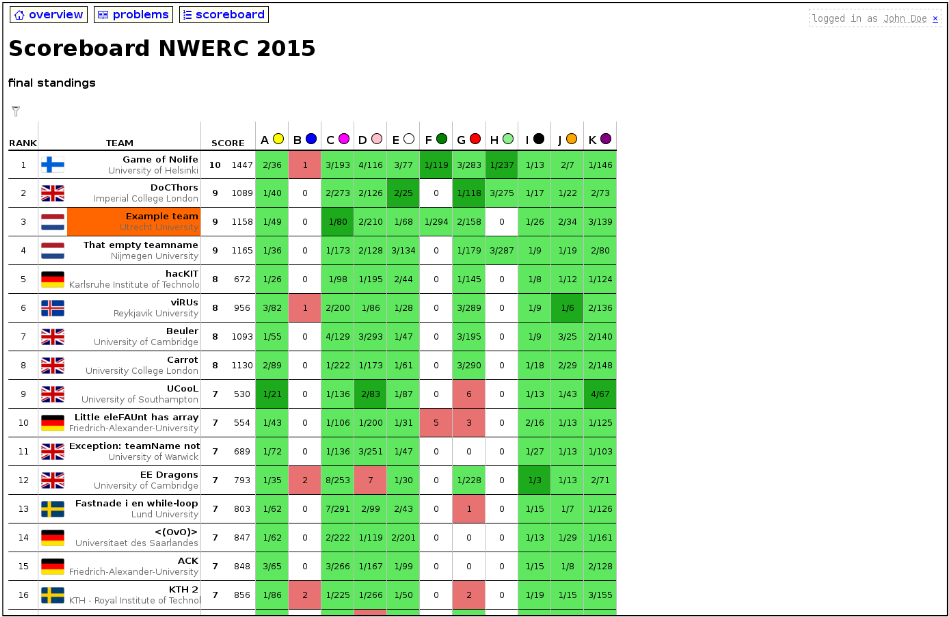
\includegraphics[scale=0.3]{scoreboard.png}
\end{center}

We are following the standard ACM-ICPC rule:

Teams are ranked according to the most problems solved. 
Teams who solve the same number of problems are ranked first by least total 
time and, if need be, by the earliest time of submittal of the last accepted 
run.

The total time is the sum of the time consumed for each problem solved. 
The time consumed for a solved problem is the time elapsed from the beginning
of the contest to the submittal of the first accepted run plus 20 penalty 
minutes for every previously rejected run for that problem. 
There is no time consumed for a problem that is not solved.

\newpage
\section{Solving a Problem}
In competitive programming contests, solving a problem takes
the following three steps:
\begin{enumerate}
    \item Read the Problem Statement
    \item Write Code and Test
    \item Submit Your Code to the Judge
\end{enumerate}

\subsection{Reading the Problem Statement}
In most programming contests, the problem statement usually
consists of several parts:
\img{0.25}{i.png}
\noindent In addition, a problem might also have a time limit and a memory limit
your program can reach at maximum:
\img{0.3}{j.png}
\noindent In conclusion, you need to read the problem statement, 
extract useful information,
understand and model the problem it asks you to solve,
and think of the approariate algorithms and data structures 
you will use later.\\\\
It is also extremely important to pay attension to the range of the input
data, as different ranges may indicate completely different algorithms
and difficulty levels for the problem.

\newpage
\subsection{Writing Code and Testing}
\subsubsection{Basics}
You write your code, compile it (for compiled languages), and test it on your
local machine.\\\\
All your code should be contained in a single source file, no matter what
language you use.\\\\
Your program should read the data from standard input, solve the problem
specified in the statement, and print the results to standard output (unless
otherwise specified).\\\\
Make sure you test your solution against the sample inputs and outputs, as it is
a bare minimum requirement for your solution to get accepted by the judge.

\subsubsection{Exit Code of Your Program}
No matter what language you use, your program should always have zero as the
exit code.\\\\
A non-zero exit code will make the judge think your program terminated in an
abnormal way, and will not accept your solution even if your output is
correct.\\\\
C++ users, please "return 0" manually in your main function. 
Python and Java users, as long as you do not call some system 
function to explicitly return a non-zero value, you should be fine.

\subsubsection{Starter Code for C++, Java and Python}
The following programs read an integer from the input, multiply it by 2
and print it to the output.\\
This should teach you what a minimal solution should look like
and how to do basic IO.\\
\begin{verbatim}
// C++
int main() // do not use void main!!!!
{
    int x;
    cin >> x;
    cout << x*2 << endl;
    return 0;
}
\end{verbatim}
\hrule
\begin{verbatim}
// Java

// do not specify any packages!!!

import java.io.*;
import java.util.*;

public class Main { // "Main" should be used for most online judges
    public static void main(String[] args) {
        Scanner sc = new Scanner(System.in);

        int x = sc.nextInt();
        System.out.printf("%d\n", x);
    }
}
\end{verbatim}
\hrule

\vspace{2pt}
We highly recommend Python users to select PyPy for Python solutions 
because PyPy is  significantly faster than the standard Python Implementation.

\begin{verbatim}
# python3
x = int(input())
print(x*2)


# python2
x = int(raw_input())
print x*2
\end{verbatim}

\newpage
\section{Understanding The Judge's Verdicts}
After your submission is received, the judge will run your
program against it's own comprehensive test cases, which are not 
visible to you, and give you a verdict.\\\\
The judge's verdict can be one of the following types:

\begin{itemize}
    \item \textbf{CORRECT}
        The submission passed all tests:  you solved this problem!
    \item \textbf{COMPILER-ERROR}
        There was an error when compiling your program.  On the submission 
        details page you can inspect the exact error.
    \item \textbf{TIMELIMIT}
        Your program took longer than the maximum allowed time for this
        problem.  Therefore it has been aborted.  This might indicate that
        your program hangs in a loop or that your solution is not efficient
        enough.
    \item \textbf{RUN-ERROR}
        There  was  an  error  during  the  execution  of  your  program.   This
        can have a lot of different causes like division by zero, incorrectly
        addressing memory (e.g.  by indexing arrays out of bounds), trying
        to  use  more  memory  than  the  limit,  etc.   Also  check  that  your
        program exits with exit code 0!
    \item \textbf{NO-OUTPUT}
        Your program did not generate any output.  Check that you write
        to standard out.
    \item \textbf{OUTPUT-LIMIT}
        Your program generated more output than the allowed limit.  The
        output was truncated and considered incorrect.
    \item \textbf{WRONG-ANSWER}
        The output of your program was incorrect.  This can happen sim-
        ply because your solution is not correct, but remember that your
        output must comply exactly with the specifications of the jury.
    \item \textbf{TOO-LATE}
        Bummer, you submitted after the contest ended!  Your submission
        is stored but will not be processed anymore.
\end{itemize}

\newpage
\section{Working With Command Line Prompt}
If you are using an EWS machine, your preferred IDE or GUI editor may not be
available. In this case, you need to switch to a text editor (vim, emacs,
sublime etc.), compile, run and test your code using the command line prompt.
\subsection{Compile and Run Your Code}
\subsubsection{C++}
\begin{verbatim}
# suppose src.cpp is your source file, use g++ to compile it
g++ src.cpp
# this will generate an executable file a.out, and you can run it by calling
./a.out

# you can use the -o option to specify the name of the executable
# otherwise, the name defaults to "a.out"
g++ src.cpp -o my_program

# if you want to use c++11, make sure to add the following option
g++ -std=c++11 src.cpp
\end{verbatim}

\subsubsection{Java}
\begin{verbatim}
# suppose Main.java is your source file, use javac to compile it
javac Main.java
# this will generate a file named "Main.class" under the same directory
# then use java to run it
java Main
\end{verbatim}

\subsubsection{Python}
\begin{verbatim}
# python is an interpreted language
# use python/python3 to run your code directly
python src.py
python3 src.py
\end{verbatim}

\newpage
\subsection{Input/Output Redirection}
Bash allows you to redirect the input and the output of a process.
This is very useful for testing as it can save you from typing 
the input data every time.\\
\begin{verbatim}
# suppose you write your input data to a text file input.txt
# then you can use < to read the data from the file and feed it to a program
my_program < input.txt

# use > to write the output of a program to a file
my_program > output.txt

# use | to pipe the output of a program to another program
ls | grep '.cpp'
\end{verbatim}

\subsection{Other Useful Commands}
\begin{verbatim}
# change the current directory to xxx
cd xxx
# the path can contain .. which means the "parent directory"
cd ../yyy

# display all the files and sub directories under the current directory
ls

# delete the file a.cpp
rm a.cpp
# delete the directory "mydir" recursively
rm -rf mydir
\end{verbatim}
\end{document}

